\chapter{Capacity Sizing with a Blended Workforce and Freelancers}

A freelancer is different from fixed as well as flexible workers. A freelancer is hired on a contract basis to serve one customer only. The contract is assumed to be binding and the freelancer immediately services the customer. Thus, the show-up probability of a freelancer is one.  \\

\section{The Need and Strategy for Hiring Freelancers} 
The question that arises now is if there is a need for hiring freelancers on top of a blended workforce. As stated in \cite{dong}, the fixed resource is used to match all or part of the demand and the flexible workers are used to match the remaining demand and to hedge against variability in capacity. However, the flexible workers might or might not show up when the shift actually starts. This variability is partially handled by employing an optimal number of flexible workers. The decision to hire flexible workers (the value of $n_{\lambda}^i$ for a shift) is taken before the shift starts by considering various factors, including their show-up probabilities. However, there is a possibility that too many flexible workers do not actually show up once the shift starts, for example, the day of a festival. Here, we propose an additional hedging strategy for a large no-show of flexible workers. Once the shift starts, the actual number of flexible workers that show up (the value of $N_{flex}(n_{\lambda}^i)$) becomes known. At this point, the manager knows the expected arrival in this shift as well as the number of available servers. He can now decide if there is a need to hire freelancers to make up for the flexible workers that didn't show up. The manager takes the decision about freelancers immediately after the start of a shift to minimize the waiting cost incurred. The trade-off would be between the cost of losing the customers and the cost of hiring the freelancers. 

\begin{remark}
Before mathematically formulating the capacity sizing problem for freelancers, some assumptions must be stated. These assumptions are in line with real-life scenarios but are stated here to avoid confusion at later stages.
\begin{itemize}
\itemsep0em
  \item The customer's abandonment time would be significantly smaller than the shift length. That is, no customers roll over to the next shift.
  \item The hiring cost of freelancers ($c_{free}$) is greater than the hiring cost for flexible or fixed workers. 
\end{itemize}
\end{remark}

\section{Optimal Staffing Strategy for Freelancers} 
Let the number of freelancers hired for a particular shift be $o_{\lambda}^i$ and the cost of hiring a freelancer is $c_{free}$. The number of fixed workers is denoted by $m_{\lambda}$, the number of flexible workers that show up for the shift are denoted by $N_{flex}(n_{\lambda}^i)$ and the length of the shift is denoted by $T_i$. The arrival process is denoted by $\Lambda$ and the arrival rate of the Poisson arrival process in period i is given by $\lambda_i$.
Then, \\
\[\text{Penalty cost per customer = Waiting time till abandonment + Abandonment cost}\]
\[\text{Expected penalty cost per customer}=\mathbb{E}(h\tau+r)\]
\[\text{Expected penalty cost per customer} =\frac{h}{\theta} + r\]
\[\text{Number of customers served by a server in shift of period $T_i$} = T_i\mu\]
\[\text{Expected number of customers that abandon the system }=\mathbb{E}((T_i\Lambda - (N_{flex}(n_{\lambda}^i) + m_{\lambda})(T_i\mu))^+)\]
\hspace{9cm} where $(x)^+=max(x,0)$
\[\text{Expected number of customers  that abandon the system }=(T_i\lambda_i - (N_{flex}(n_{\lambda}^i) + m_{\lambda})(T_i\mu))^+\]
Hiring should happen so that cost of hiring does not exceed the cost of losing customers. Thus, 
\[o_{\lambda}^i.c_{free}\leq (\frac{h}{\theta} + r).(T_i\lambda_i - (N_{flex}(n_{\lambda}^i) + m_{\lambda})(T_i\mu))^+\]
\[o_{\lambda}^i = \left \lfloor{\frac{(\frac{h}{\theta} + r).(T_i\lambda_i - (N_{flex}(n_{\lambda}^i) + m_{\lambda})(T_i\mu))^+}{c_{free}}}\right \rfloor \]

\begin{remark}
If enough servers are available to meet the expected arrivals once the shift starts, our solution will not install any capacity, as is expected. Mathematically, 
\[T_i\lambda_i \leq (N_{flex}(n_{\lambda}^i) + m_{\lambda})T_i\mu \implies (T_i\lambda_i - (N_{flex}(n_{\lambda}^i) + m_{\lambda})T_i\mu)^+=0 \implies o_{\lambda}^i=0\]

\end{remark}

\section{Numerical Results}
For our numerical analysis, we are considering a 2-shift model with one shift being a low-demand period with $\lambda_1=25$ and other high demand period with $\lambda_2=50$. We take that shifts are of length $T_1=2$ and $T_2=1$ , where $T_i$ is the time period of shift $i$. We assume that the distribution for $\epsilon$ is uniform on $(-1,1)$ and that of server showup is binomial with $p=0.8$ and the value of $a=1$. We take that $h=r=1$ and $\mu=1,\theta=0.5$.The costs for employing servers are $c_{fix}=2/9,c_{flex}=1/3,c_{free}=0.35$. We are taking $q$ from $0.2$ to $1$ in increments of $0.01$.
\\ To observe the workings of our blended workforce model, we need to look at two perspectives , the firm perspective and the customer perspective
\subsection{Firm Perspective : Cost Reduction}
From the Figure 6.1, we can see that the cost is lowest for the blended force, which grows closer to fixed cost as $q$ increases because we are employing more number of flexible workers to hedge the uncertainty.We can also see that the freelancers are adding an extra cost which is expected as we are employing freelancers for Quality of service but not cost reduction. Even with the added cost, the model with freelancers is cheaper when compared to just flexible or fixed when there is moderate to high certainty.
\\\begin{figure}[hbt!]
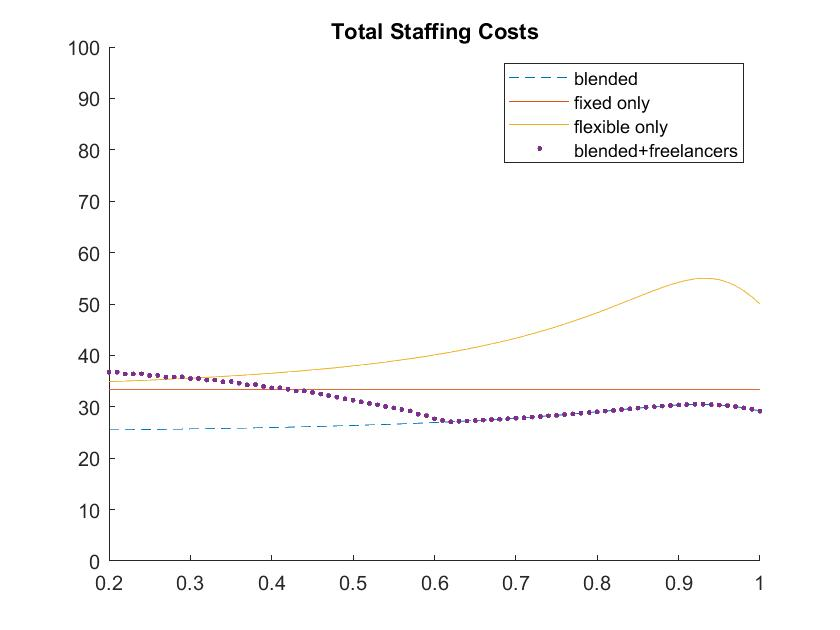
\includegraphics[height=10cm]{cost.jpg}
\caption{Total Staffing Costs}
\subcaption{This image shows the total staffing costs, that is for both the periods (high and low-demand) for different types of work forces.}
\end{figure}
\subsection{Customer Perspective : Quality of Service}
To observe the quality of service, we are looking at the expected number of customers being abandoned. 
\\We can see that in the low demand period that blended and blended+freelancer are the same as we are not employing any freelancers because the system is already overstaffed, and we can see that as the uncertainty increases we are over-staffing the system more and more hence increasing the quality but trading it off with the cost. 
\\For the high demand period, employing freelancers is helping us in increasing in the quality of service when compared to  blended or just flexible. We can also see that as $q$ increases, we are over-staffing with flexible to hedge the uncertainty so we are not hiring any freelancers and the two plots merge.
\\\begin{figure}[hbt!]
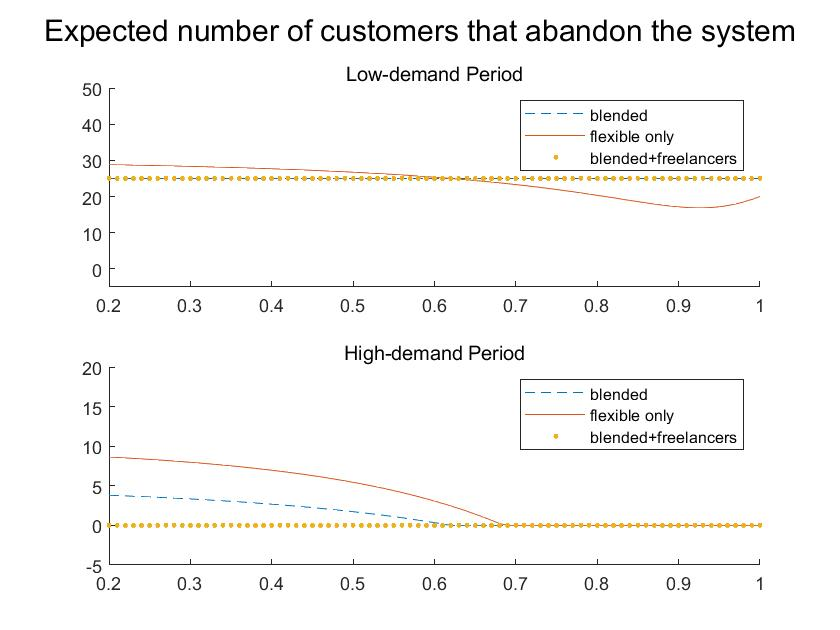
\includegraphics[height=10cm]{abandon.jpg}
\caption{Expected number of customers that abandon the system for p=0.8}
\subcaption{This image shows the number of customers that are expected to leave the system in the 2 different periods. }
\end{figure}
\\
It is clear that the aim of adding freelancers is improving the quality of service by hedging against less show-up of flexible workers while trading off efficiency. When the show-up probability is as high as 0.8, we still see an improvement in quality of service with freelancers. We now explore the degree of improvement of quality of service for other show-up probabilities. We focus on the analysis of blended vs blended+freelancer regimes in the following sections.
\subsubsection{Improvement in the Quality of Service when the show-up probability is high}
Figure 6.3 represents this case. \\ In the low-demand period, the number of flexible workers hired remains low, as a result, freelancers required to hedge the less show-up of flexible workers is very low (0 in this case). There is no improvement in the quality of service by adding freelancers but there is no loss in terms of efficiency because they are not being hired.\\ In the high-demand period, we see a difference. Flexible workers would now be hired to supplement the fixed workforce. In the variability-dominated and a large part of the moderately uncertainty-dominated regimes, we see that the adding of freelancers improves the quality of service by reducing the number of customers abandoning the system. Once the value of $q$ exceeds 0.5, no freelancers are hired, and hence, there is no improvement in the quality of service. This happens because the manager hires high number of flexible workers because he knows that there is high variability in their show-up. Thus, the hiring of large number of flexible workers hedges the less show-up situation, and freelancers are not needed.
\subsubsection{Improvement in the Quality of Service when the show-up probability is moderate}
We keep all the parameters same as the previous case but change the show-up probability, $p$, to $0.5$. \\
\begin{figure}[hbt!]
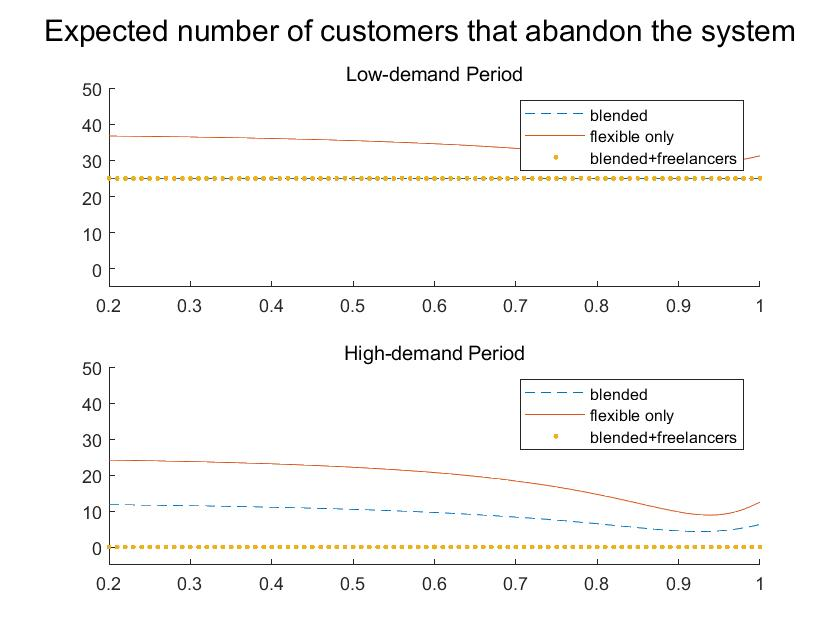
\includegraphics[height=10cm]{p0.5.jpg}
\caption{Expected number of customers that abandon the system for p=0.5}
\subcaption{This image shows the number of customers that are expected to leave the system in the 2 different periods. }
\end{figure}
Figure 6.5 represents this case. \\ In the low-demand period, the results are just like in the case of p=0.8. The number of flexible workers hired remains low, as a result, freelancers required to hedge the less show-up of flexible workers is very low (0 in this case). There is no improvement in the quality of service by adding freelancers but there is no loss in terms of efficiency because they are not being hired.\\ In the high-demand period, we see a difference. Flexible workers would now be hired to supplement the fixed workforce. Across all regimes (from $q=0.2$ to $q=1$), we see that the adding of freelancers improves the quality of service by reducing the number of customers abandoning the system. 
\subsubsection{Improvement in the Quality of Service when the show-up probability is low}
We keep all the parameters same as the previous case but change the show-up probability, $p$, to $0.2$. \\
\begin{figure}[hbt!]
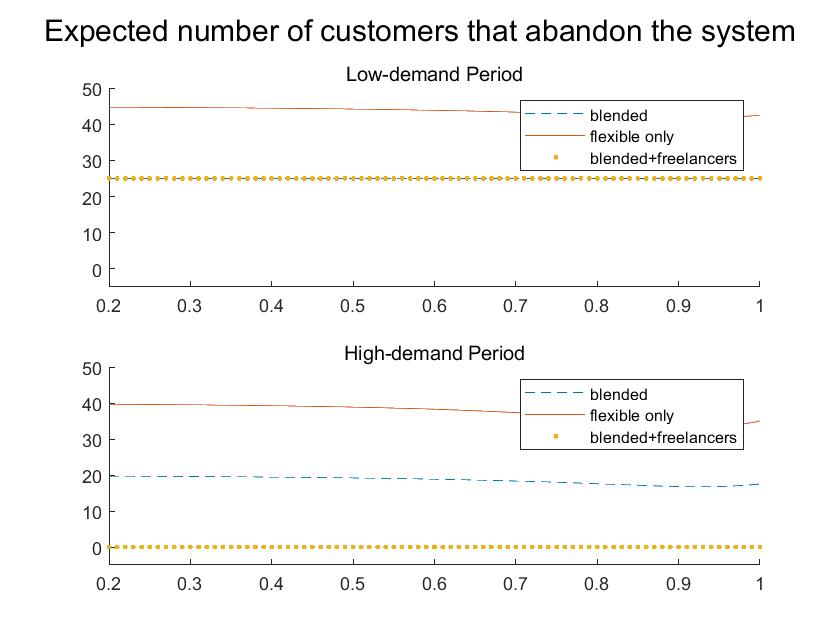
\includegraphics[height=10cm]{p0.2.jpg}
\caption{Expected number of customers that abandon the system for p=0.2}
\subcaption{This image shows the number of customers that are expected to leave the system in the 2 different periods. }
\end{figure}
Figure 6.7 represents this case. \\ In the low-demand period, the results continue to remain the same because the number of flexible workers hired remains low, and as a result, freelancers required to hedge the less show-up of flexible workers is very low. \\ In the high-demand period, we see a trend very similar to the case when $p=0.5$. Across all regimes (from $q=0.2$ to $q=1$), we see that the adding of freelancers improves the quality of service by reducing the number of customers abandoning the system. The trend remains the same but the gap between the expected number of customers abandoning the system for the blended vs blended+freelancers case widens.
\subsection{Combining both perspectives}
In our addition to the model, we are more focused on improvement of quality of service, as we feel in real life, with the increased competition in the market, the emphasis has been shifting to quality of service. So, combining both the firm and customer perspective with an emphasis on quality of service, we can divide our model into mainly 3 regimens
\\ \textbf{ \textit {(I) [Variability-dominated.]}} In this regime, we can see that the quality of service is best in the model with freelancers, but we can also see that the cost is very high and when we have high to moderate show-up probability for the flexible workers, the change in quality of service is not that substantial with the addition of freelancers, so for this regime, the best strategy would be to have a blended workforce without freelancers, when you have moderate to high show-up probabilities and only employ freelancers when you expect low probability of showing up.
\\ \textbf{ \textit {(II) [Moderately uncertainty-dominated.]}}
It is in this regime that we can see the workings of freelancers, the cost is lower with freelancers, when compared to just flexible or just fixed and though the cost is slightly higher when compared to blended, we can see that quality of service is greatly improved. So for this regime, the best strategy would be a blended+freelancer model.
\\ \textbf{ \textit {(III) [Strongly uncertainty-dominated.]}}
In this regime we are not employing any freelancers as we already hedge the uncertainty with a  high number of flexible workers and we can see that here we have almost the same cost for blended and fixed. In this case, we could see that blended is optimal.